\documentclass[12pt,letterpaper]{article}
\usepackage{fullpage}
\usepackage[top=1.5cm, bottom=3.5cm, left=2.2cm, right=2.2cm]{geometry}
\usepackage{amsmath,amsthm,amsfonts,amssymb,amscd, esint}
\usepackage{lastpage}
\usepackage{enumerate}
\usepackage{fancyhdr}
\usepackage{mathrsfs}
\usepackage{graphicx}
\usepackage{listings}
\usepackage{hyperref}
\usepackage[english]{babel}
\usepackage{lipsum}
\usepackage[table,xcdraw]{xcolor}
\usepackage{enumitem}
\usepackage{float}
\usepackage{chemfig}
\usepackage{yfonts}
\usepackage{braket}
\usepackage{dsfont}
\usepackage{tikz}
\usepackage{wrapfig}
\usepackage{url}
\usepackage{natbib}
\usepackage[normalem]{ulem}
\usepackage{multicol}
\useunder{\uline}{\ul}{}


%%%%%%%%%%%%%%% CODELISTINGS %%%%%%%%%%%%%%%%
\usepackage{listings}
\definecolor{codegreen}{rgb}{0,0.6,0}
\definecolor{codegray}{rgb}{0.5,0.5,0.5}
\definecolor{codepurple}{rgb}{0.58,0,0.82}
\definecolor{backcolour}{rgb}{0.95,0.95,0.92}

\lstdefinestyle{mystyle}{
    backgroundcolor=\color{backcolour},   
    commentstyle=\color{codegreen},
    keywordstyle=\color{magenta},
    numberstyle=\tiny\color{codegray},
    stringstyle=\color{codepurple},
    basicstyle=\ttfamily\footnotesize,
    breakatwhitespace=false,
    breaklines=true,                 
    captionpos=t,                    
    keepspaces=true,                 
    numbers=left,                    
    numbersep=5pt,                  
    showspaces=false,                
    showstringspaces=false,
    showtabs=false,                  
    tabsize=2
}

\lstset{style=mystyle}

%%%%%%%%%%%%%%%%%%%%%%%%%%%%%%%%%%%%%%% 
\usepackage{titlesec}
\usepackage{textcase} % for uppercase handling

% --- Section formatting ---
\titleformat{\section}
  {\normalfont\normalsize\bfseries\centering} % font size, bold, centered
  {\thesection}{1em}{\MakeTextUppercase} % uppercase text

% --- Subsection formatting ---
\titleformat{\subsection}
  {\normalfont\large\bfseries\centering}
  {\thesubsection}{1em}{\MakeTextUppercase}

% --- Roman numerals for numbering ---
\renewcommand{\thesection}{\Roman{section}}
\renewcommand{\thesubsection}{\Roman{section}.\roman{subsection}}

\newtheorem{definition}{Definition}
\newtheorem{observation}{Observation}
\newtheorem{reflection}{Reflection}
\newtheorem{PyPackage}{Package}
\newtheorem{book}{Book}

\newcommand{\HRule}[1]{\rule{\linewidth}{#1}}
\setcounter{tocdepth}{5}
\setcounter{secnumdepth}{5}

\setlength{\parindent}{0.0in}
\setlength{\parskip}{0.05in}

% Edit these as appropriate
\newcommand\course{}
\newcommand\subject{Final Degree Project}
\newcommand\degree{Bachelor's Degree in Physics}
\newcommand\documenttitle{Lower bounds of the success probability in quantum state exclusion for general ensembles}
\newcommand\NetIDb{Universitat Autònoma de Barcelona}
\newcommand\AuthorName{Sergio Castañeiras Morales}

\hypersetup{%
  pdftitle  = \documenttitle,
  pdfauthor = \AuthorName,
  pdfsubject= \degree,
  pdfcreator= \AuthorName,
}

\usepackage{glossaries}
\usepackage{glossary-longragged}

\makenoidxglossaries
\newacronym{qse}{QSE}{Quantum State Exclusion}
\newacronym{qsd}{QSD}{Quantum State Discrimination}
\newacronym{sdp}{SDP}{Semidefinite Program}
\newacronym{povm}{POVM}{Positive Operator-Valued Measure}
\newacronym{me}{ME}{Minimum Error}
\newacronym{ze}{ZE}{Zero Error}
\glsaddall[types=\acronymtype] 

\DeclareMathOperator{\tr}{Tr}


\begin{document}
\title{\vspace{4cm} \normalsize 
		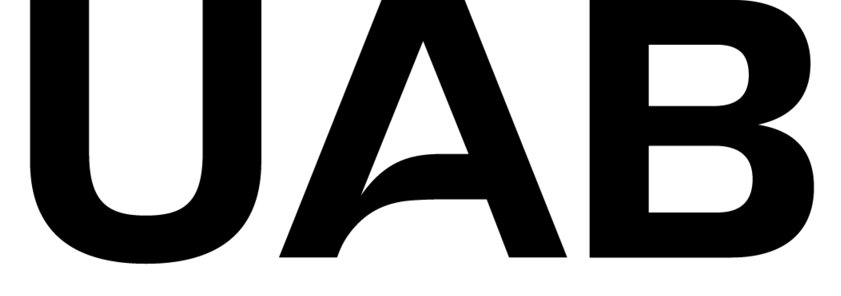
\includegraphics[width = 0.25\textwidth]{GeneralSources/UABLogo.png}\\ [0.5cm]
		\textsc{\NetIDb}\\ [2.0cm]
		\HRule{0.5pt} \\
		\LARGE \textbf{\uppercase{\documenttitle}}
		\HRule{2pt} \\ [1.5cm]
		\normalsize \begin{tabular}{rcl}  % Create a right-left column alignment
        \textsc{Author} & : & \textsc{\AuthorName} \\
        \textsc{Supervisor} & : & \textsc{Ramón Muñoz Tapia} \\
        \textsc{Co-Supervisor} & : & \textsc{Santiago Llorens Fernández}
    \end{tabular}
    \normalsize \vspace*{5\baselineskip}
		}

\date{2024-2025}

\author{\large \textsc{\subject} \\ \textsc{\degree}}



\begin{titlepage}
\clearpage\maketitle
\thispagestyle{empty}
\end{titlepage}

\thispagestyle{empty}
\mbox{} 
\newpage
\thispagestyle{empty}
\vspace*{\fill} % Push content to vertical center
\begin{flushright}
    \emph{Ab ovo usque ad mala.}\\[1em]
    \textbf{Horace}
\end{flushright}
\vspace*{\fill} 
\newpage

\newpage
\pagestyle{fancyplain}
\headheight 35pt
\lhead{\NetIDb}    
\rhead{\subject}
\cfoot{\small\thepage}
\headsep 1.5em

\begin{multicols}{2}[\begin{center}
\begin{abstract}
Given a quantum state known to be prepared from an ensemble of two or more states, quantum state exclusion aims to rule out the possibility that it was prepared in a particular state from the ensemble. Using the known solution for group generated ensembles \cite{MainPaper}, we study this result as a lower bound for randomly generated ensembles via semidefinite programming.
\end{abstract}
\end{center}
Keywords: \emph{SDP, Quantum state exclusion , \textcolor{blue}{Add keywords}}.
]
\section{Introduction}
\vspace{-0.5cm}
In many real-world scenarios, excluding a certain hypothesis can be more practical than solving the problem entirely. For instance, in disease diagnosis, ruling out potential diseases often serves as the first step in identifying the actual condition. Similarly, when repairing a machine, it is sometimes more efficient to identify the components that are functioning correctly, which narrows down the search for the faulty part.

In this project, we project this idea into the quantum realm by focusing on \gls{qse}. Rather than determining the exact state of a quantum system, we aim to eliminate one or more possible candidates from a known ensemble of states. Notice, this approach can be more suitable or efficient in certain quantum information tasks.

Given a quantum state known to be prepared from a finite ensemble, \gls{qsd} seeks to identify which specific state from the ensemble corresponds to the given system. In contrast, \gls{qse}~\cite{PhysicsExclusionSource} adopts the opposite perspective: it aims to determine which states from the ensemble do not correspond to the prepared state. While \gls{qsd} has been deeply studied in recent years\cite{DiscriminationArticle}, with significant advances since its inception~\cite{helstromBook}, \gls{qse} offers a complementary framework with distinct advantages.

Although the tasks of exclusion and discrimination coincide for ensembles containing only two states \footnote{Since for the two states case excluding one necessarily implies identifying the other.}, when dealing with ensembles of three or more states, the two problems diverge in both approach and complexity. One of the most significant features of \gls{qse} is the possibility of achieving \emph{perfect exclusion}, where certain states can be ruled out with zero probability of error in cases where perfect discrimination is impossible\cite{OptimalitySRM}. 

This capability opens new frontiers in quantum information theory, particularly in the context of partial information retrieval from quantum systems. By excluding certain states, it is possible to gain insight into the encoded information without needing to fully determine the original state.

As with \gls{qsd}, obtaining a general analytical solution for \gls{qse} remains an open problem. However, analytical results have been found in specific cases when the ensemble of quantum states exhibits a certain degree of symmetry. In particular, when the ensemble is generated by the action of a finite group, the problem becomes more tractable and exact solutions have been derived.

The exclusion task can be carried out under two main protocols: \emph{Minimum Error} and \emph{Zero Error}\footnote{Also known as \emph{unambiguous exclusion}.}. In the Minimum Error scenario, the goal is to minimize the probability of mistakenly excluding the actual prepared state. In contrast, the Zero Error approach seeks to exclude a state with absolute certainty, even if that means sometimes the procedure yields an inconclusive result.

Building on recent results that provide exact solutions for exclusion tasks in group generated ensembles \cite{MainPaper}, this project undertakes a numerical study of such results as lower bounds for more general, randomly generated ensembles. To this end, we employ \gls{sdp} to explore \gls{qse} performance in arbitrary settings. Furthermore, we investigate improved bounds for the general case based on how closely a given ensemble resembles a group-generated one\footnote{The notion of "how close" will be formally defined in Section~\textcolor{blue}{add section}.}.

\vspace{-0.5cm}
\section{Formulation of the problem}
\vspace{-0.5cm}
Let $\left\{(\rho_i,\eta_i)\right\}_{i=1}^n$ be a set of $n$ states and $n$ probabilities, where $\rho_i$ dennotes the density matrix $\rho_i=\ket{\psi_i}\bra{\psi_i}$, and $\eta_i$ dennotes the prior probability in which $\rho_i$ accours. Additionally, let $\rho_j$ be a state belonging to the ensemble be our target state, we aim to develope a proceadure to find $\rho_k\in\left\{\rho_i\right\}_{i=1}^n$ such that $\rho_j\neq\rho_k$.

The quantum mesurement is represented by a \gls{povm} set dennoted as $\left\{\Pi_j\right\}_j$ acting on quantum states' Hilbert space $\mathcal{H}$. 

Hence, the formulation in a \gls{sdp} problem for the \gls{me} protocol for the miminization of the probability of excluding our target state from our hypothesis in the minimum error protocol reads,
\begin{align*}
	P_{\text{\gls{me}}}^e=\min_{\Pi_i}&\sum_{i=1}^n\tr{(\Pi \rho_i)},\\
	\text{subject to }&\sum_{i=1}^n \Pi_i = \mathds{1},\Pi_i\geq0 \hspace{0.5cm}\forall i\in\set{1,...,n}
\end{align*}

notice that both conditions $\sum_{i=1}^n \Pi_i = \mathds{1}$ and $\Pi_i\geq0$ stands for the \gls{povm} definition i.e. by demanding possible definitness and a sum equal to the identity we are demanding $\left\{\Pi_j\right\}_j$ to be a set of \gls{povm}s. Notice the $e$ upperindex stands for the \emph{error probability}.

Similarly the problem can trivially be formulated in an equivalent way in terms of the maximization of the \emph{success probability}, defined as the probabilty of a successfull exclusion form the point of view

\begin{align*}
	P_{\text{\gls{me}}}^s=\max_{\Pi_i}1-&\sum_{i=1}^n\tr{(\Pi \rho_i)},\\
	\text{subject to }&\sum_{i=1}^n \Pi_i = \mathds{1},\Pi_i\geq0 \hspace{0.5cm}\forall i\in\set{1,...,n}
\end{align*}
Since naturally, $P_{\text{\gls{me}}}^s+P_{\text{\gls{me}}}^e = 1$.

Moreover we refere an ensemble as a \emph{group generated ensemble} when it is the outcome of one or more unitary transformations $U_i$ applied onto a seed state such that $U_i$ generates a finite group. For instance if $U_i^n=\mathds{1}$ will lead up a $\mathbb{Z}/n\mathbb{Z}$ group generated ensemble. 
%%%%%%%%%%%%%%%%%%%%%%%%%%%%%%%%%%%%%%%%%%
%%%%%%%%%%%%%%%% BIBLIOGRAPHY %%%%%%%%%%%%%%%%%
%%%%%%%%%%%%%%%%%%%%%%%%%%%%%%%%%%%%%%%%%%

\bibliographystyle{plain}
\bibliography{references} 
%%%%%%%%
\section*{List of abbreviations}
\renewcommand{\glsnamefont}[1]{\textbf{#1}}
\printnoidxglossary[type=main, title={\vspace{-1cm}}, nonumberlist, nogroupskip, style=super]


\end{multicols}
\end{document}
